% insert plot figure2
\begin{figure}[h]
    \centering
    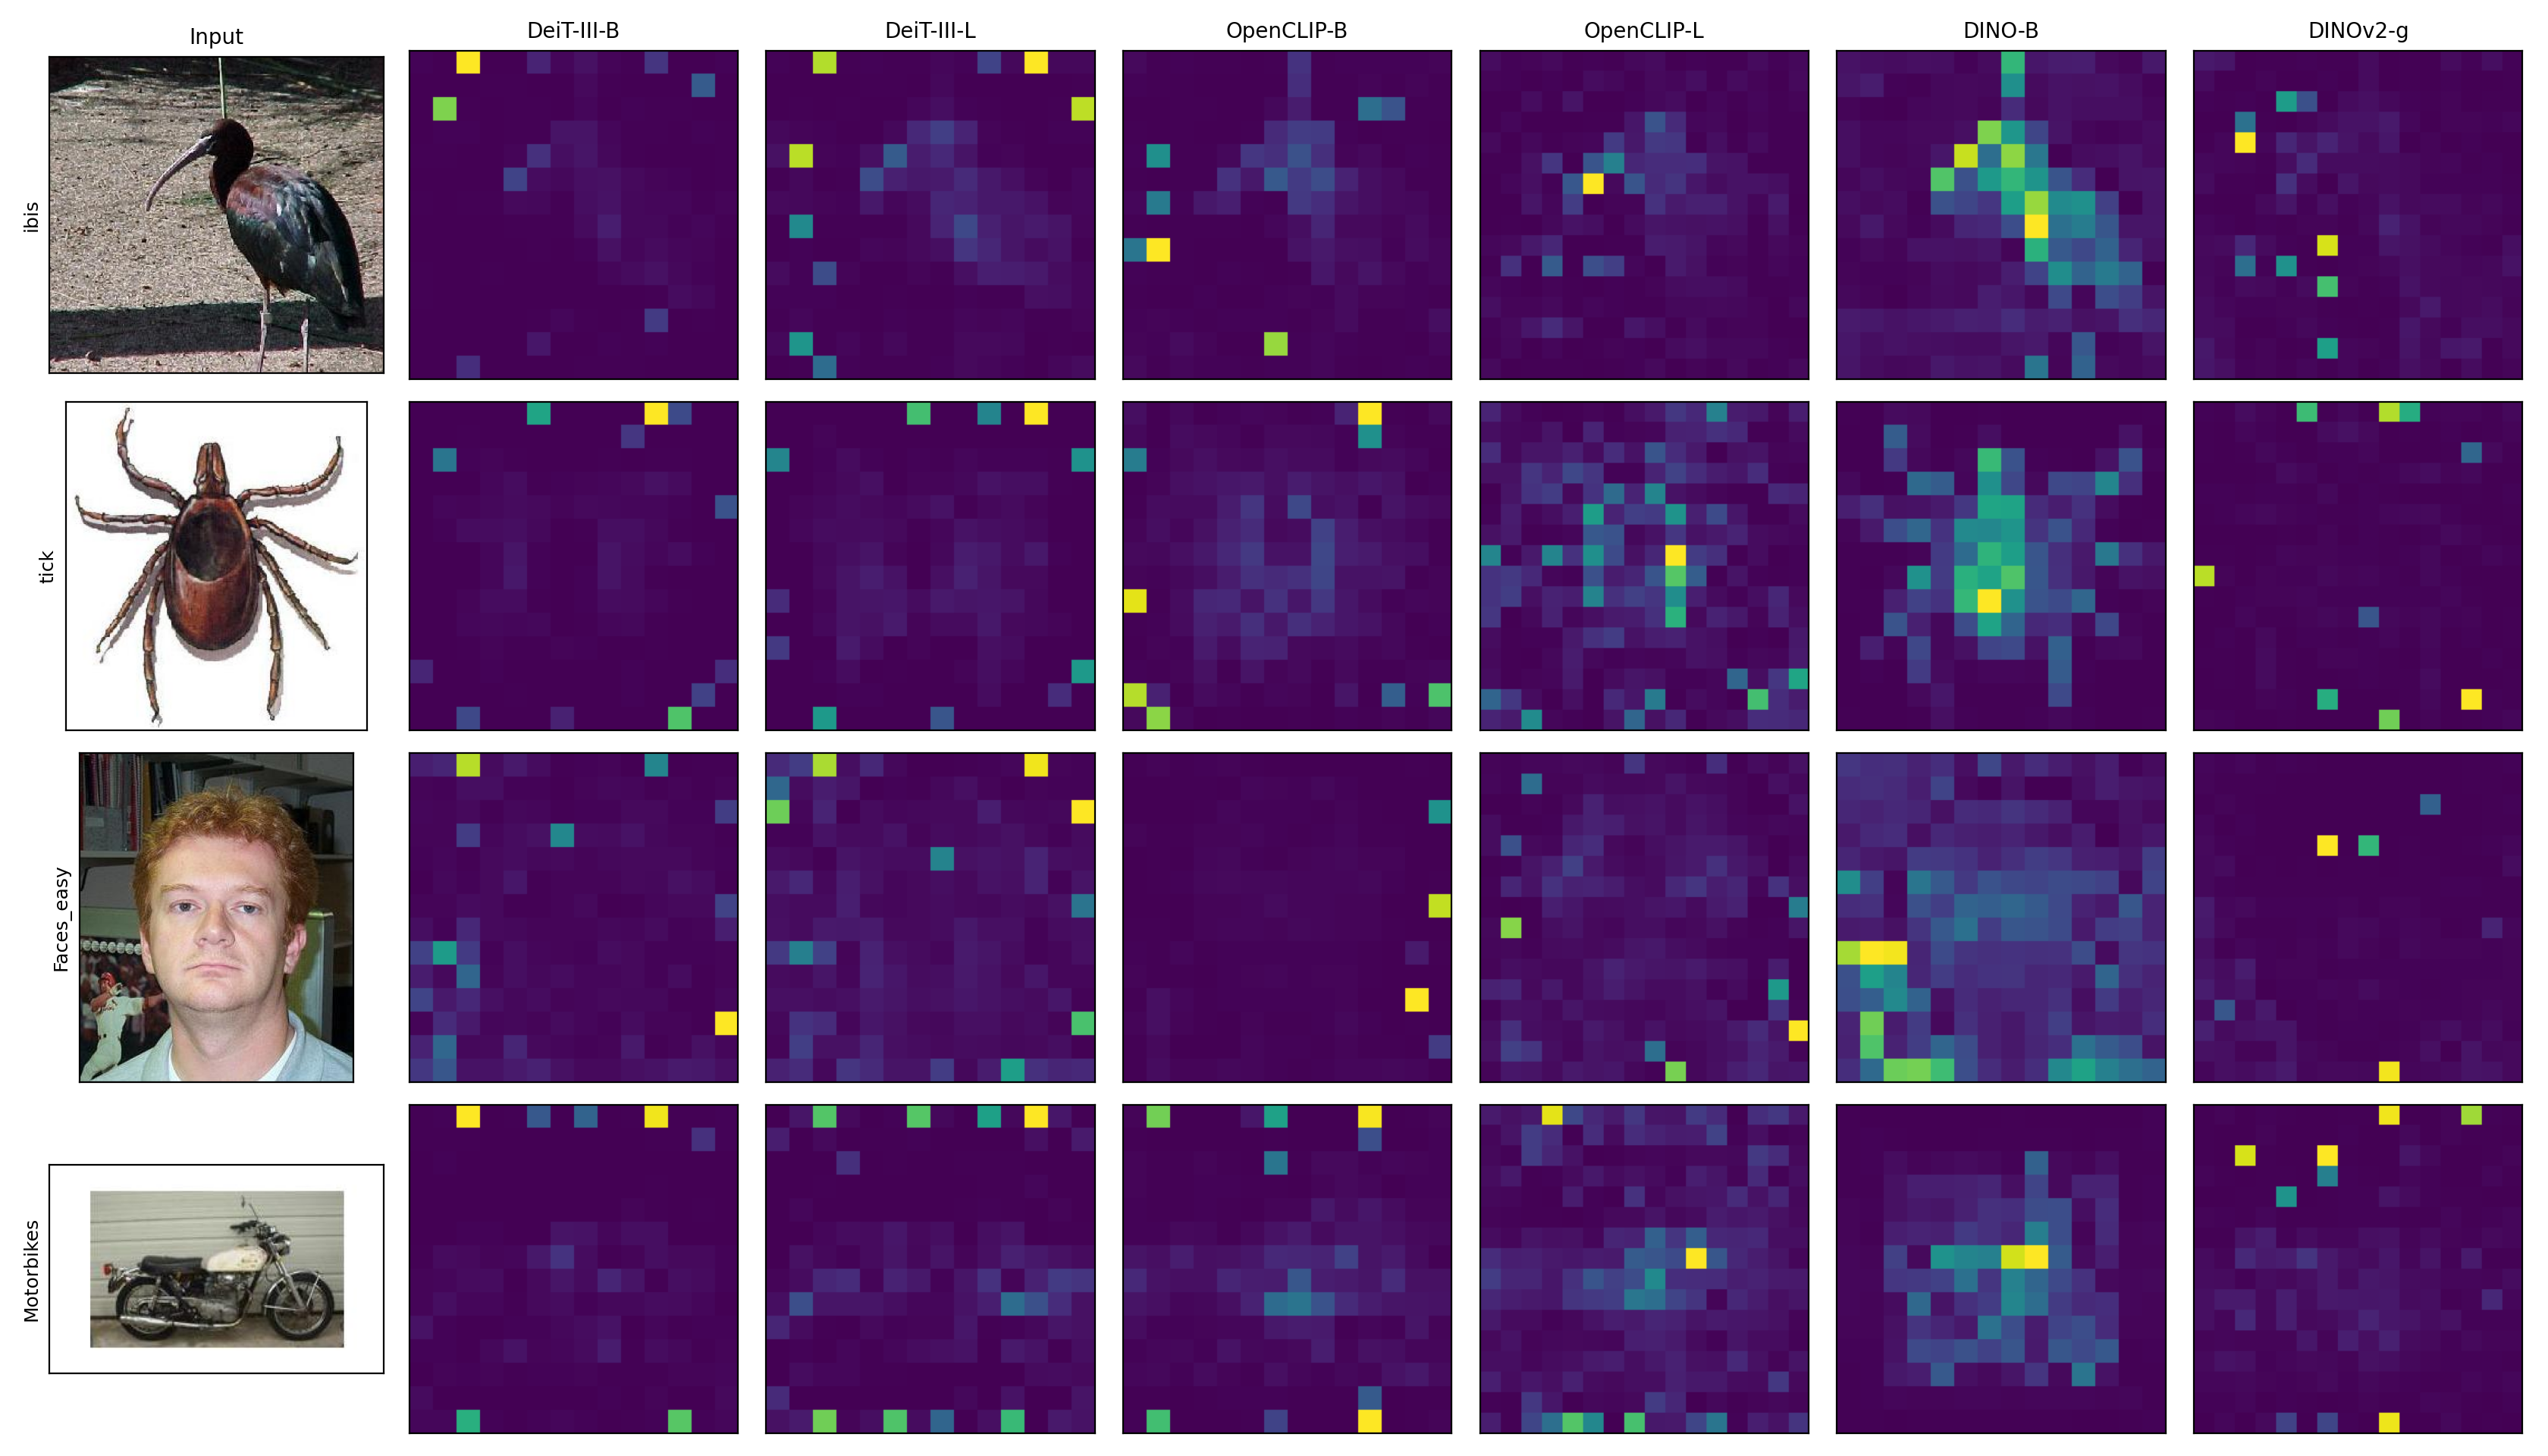
\includegraphics[width=0.7\textwidth]{../../src/Kun/img/figure2_att_map.png}
    \caption{Attention maps for 6 different model families.}
    \label{fig:outlier_maps}
\end{figure}

% insert plot figure3
\begin{figure}[h]
    \centering
    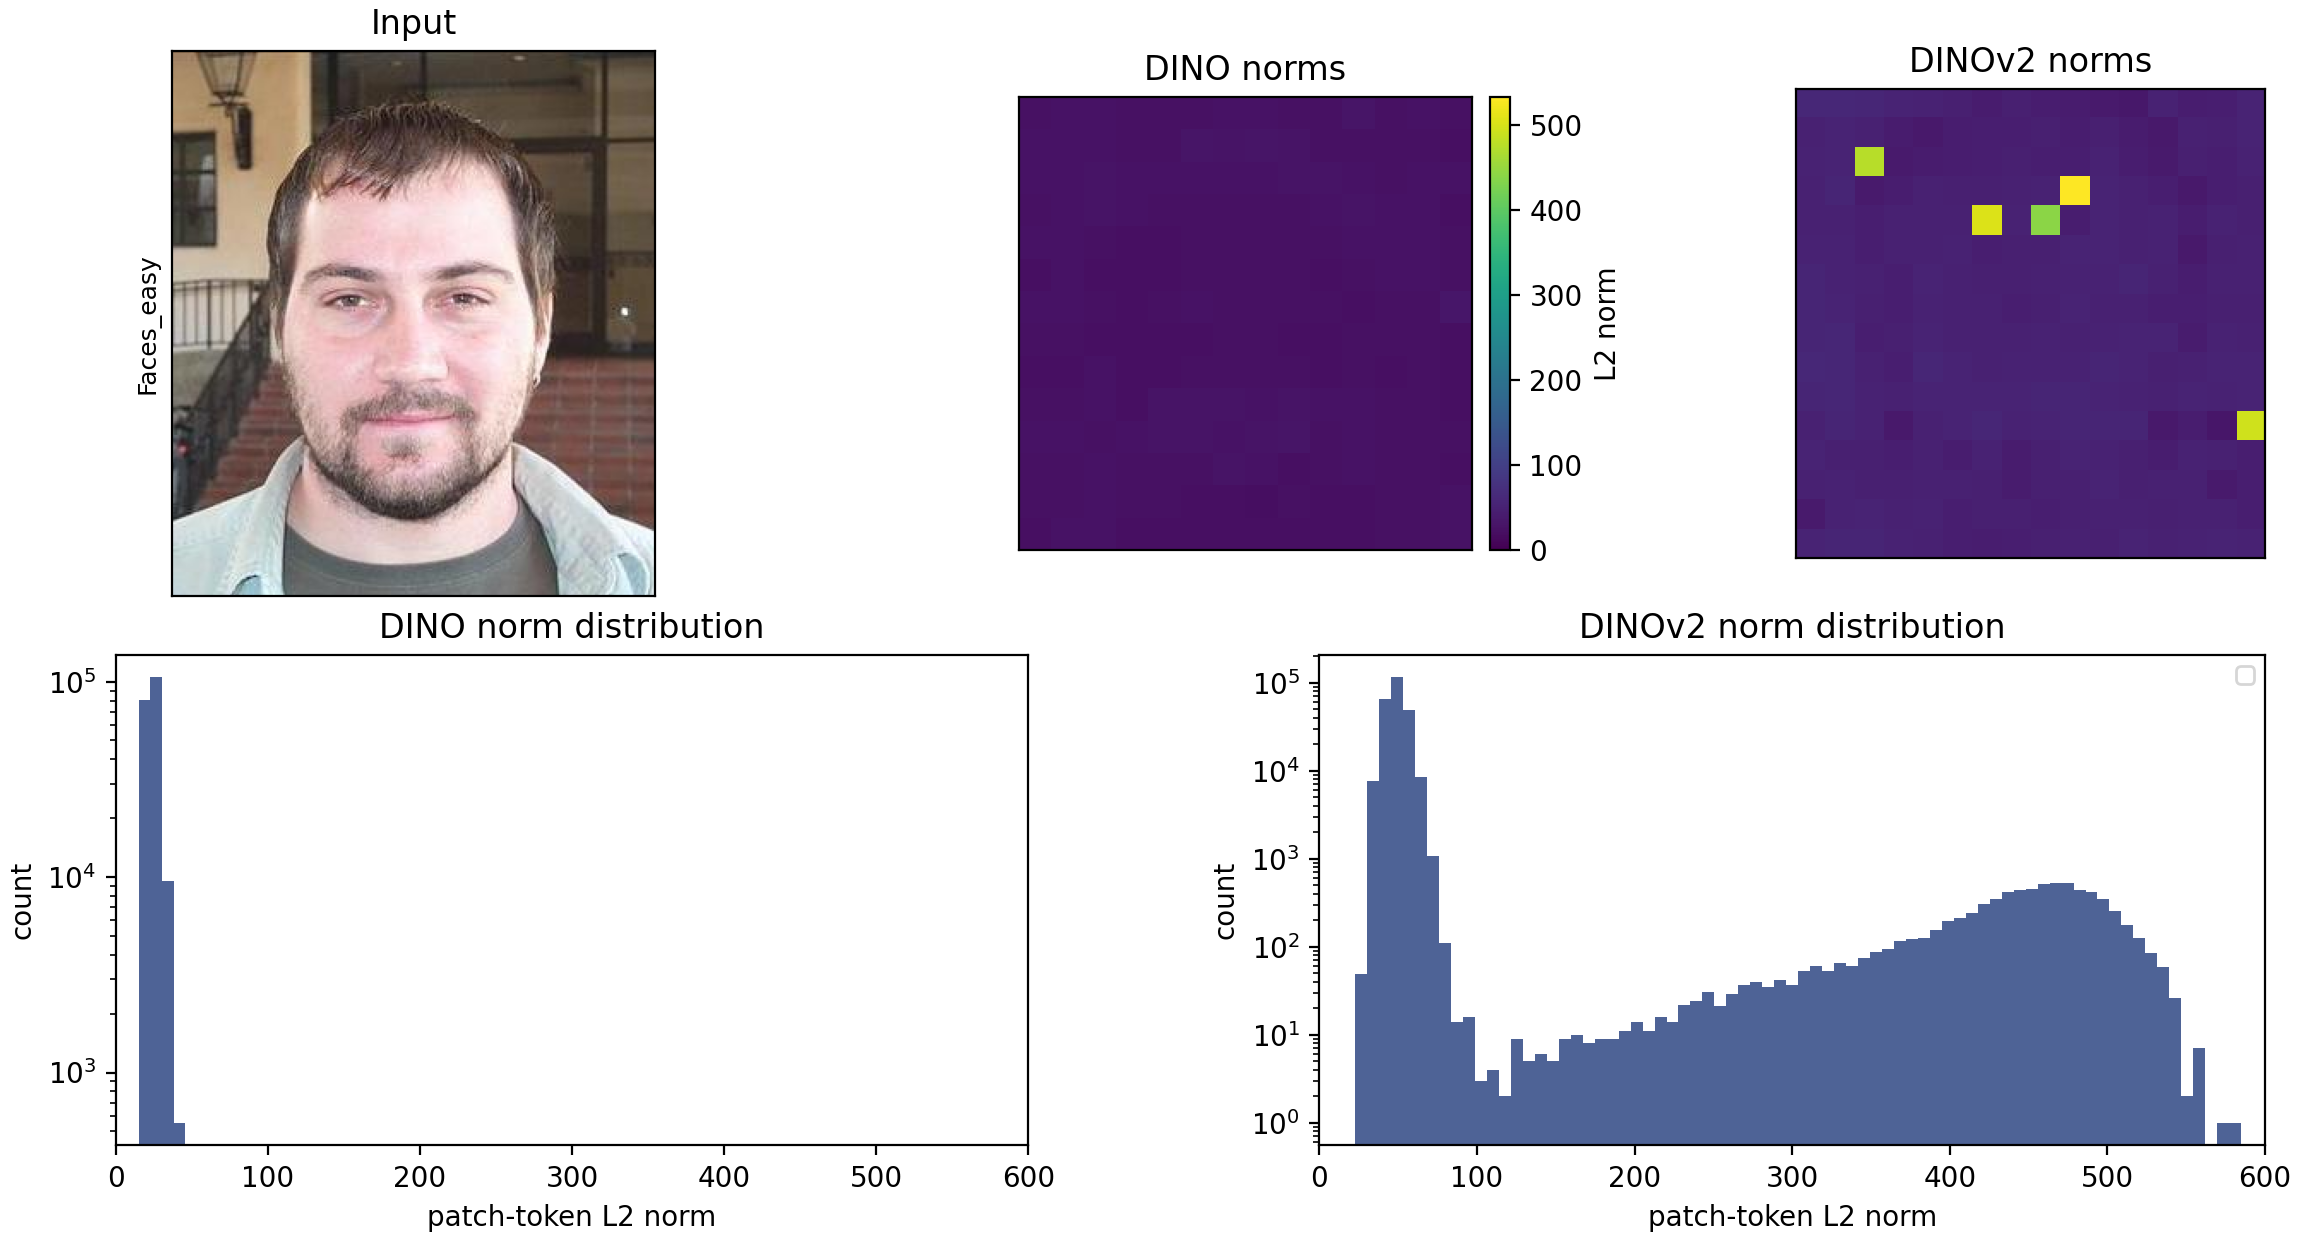
\includegraphics[width=0.7\textwidth]{../../src/Kun/img/figure3_norms.png}
    \caption{Norm distribution of local features for DINO and DINOv2.}
    \label{fig:dino_vs_dinov2}
\end{figure}

% insert figure5a 5b
\begin{figure}[h]
    \centering
    \begin{minipage}{0.3\textwidth}
        \centering
        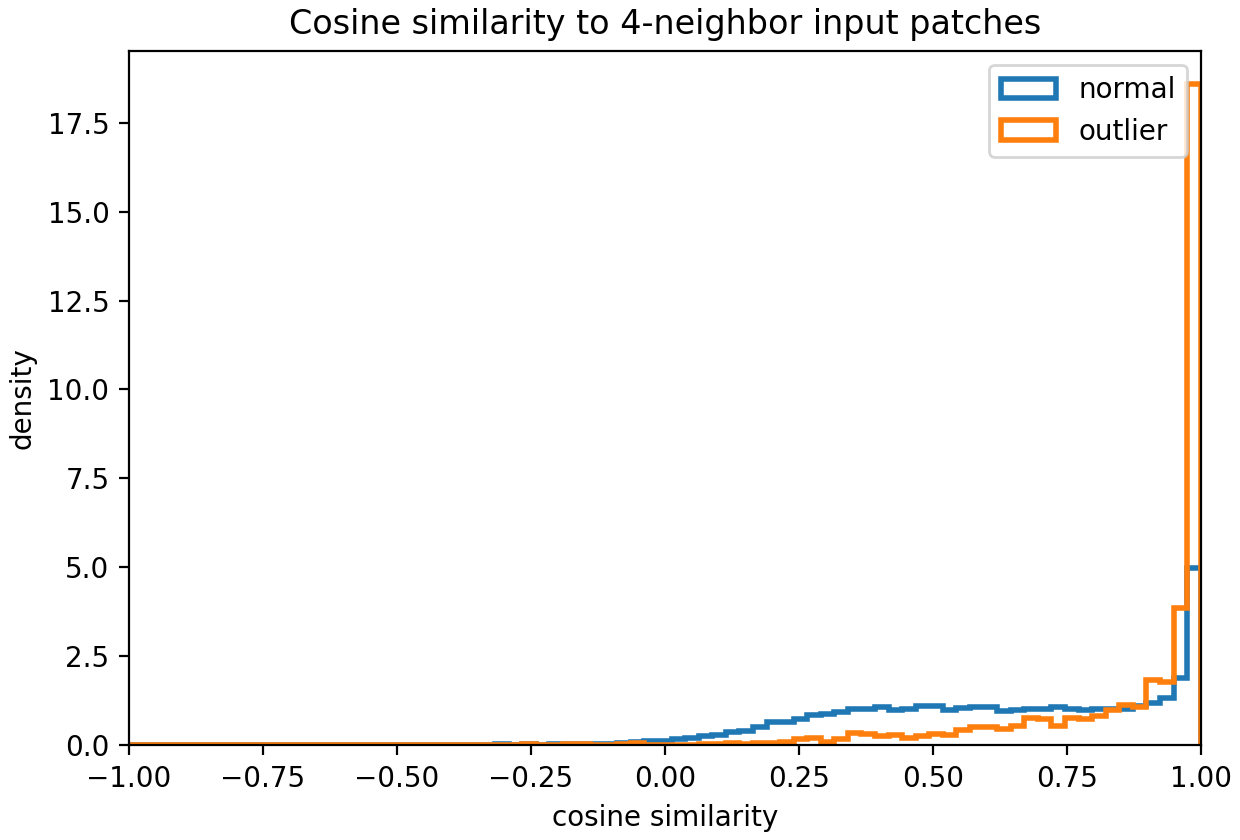
\includegraphics[width=\textwidth]{../../src/Kun/img/figure5a_neighbor_cosine.png}
    \end{minipage}\hspace{0.02\textwidth}
    \begin{minipage}{0.4\textwidth}
        \centering
        \footnotesize
        \label{tab:local_probe}
        \resizebox{\linewidth}{!}{%
        \begin{tabular}{lccc}
            \toprule
            Token group & Position top-1 acc. (\%) & Avg. distance & Reconstruction $L_2$ error \\
            \midrule
            Normal  & 19.4 & 1.19 & 17.78 \\
            Outlier & 9.7  & 5.92 & 22.64 \\
            \bottomrule
        \end{tabular}
        }
    \end{minipage}
    \caption{local information probing: cosine similarity of outlier/normal patches to their neighbors (left) and local probe results (right).}
    \label{fig:neighbor_cosine}
\end{figure}
